\documentclass[12pt]{article}
\usepackage[T1]{fontenc}
\usepackage[polish]{babel}
\usepackage[utf8]{inputenc}
\usepackage{graphicx}

\graphicspath{ {./images} }


\title{Zadanie numeryczne 2}
\author{Jakub Heczko}
\date{}

\begin{document}
\maketitle
\section{Wstęp}
W drugim zadaniu numerycznym musieliśmy wyliczyć oraz naszkicować wykres błedu funkcji, która liczyła bład z pochodnej w punkcie używając ilorazu różnicowego i "normalnej" ręcznie obliczonej pochodnej.
\newline
Na początku przedstawie jak wyglądają wykresy dla punktu x = 1 w którym obliczamy pochodną i omówie wyniki dla kazdego z nich. Pierwszy rysunek, to są wykresy dla double, a drugi rysunek dla float.
\section{Omowienie dla precyzji float i double oraz punktu x = 1}
\subsection*{Double}
\includegraphics[width=15cm,height=10cm, keepaspectratio]{wykres_double_1}
\subsection*{Float}
\includegraphics[width=15cm,height=10cm, keepaspectratio]{wykres_float_1}
\subsection{Analiza ilorazu A}
Najpierw zastanówmy się skąd wynika błąd na pierwszym wykresie(to jest pierwszy rysuenek, Iloraz A), pierwszy rodzaj błedu z jakims mamy do czynienia, to fakt, ze uzywamy skończonej arytmetyki, co sprawia, ze nasze liczby są obarczone jakimś błędem przyblizenia, drugi blad, to fakt, ze chcemy policzyc "skonczona granice". Sprawia to, ze zawsze nasza granica bedzie niedoskonała i obarczona błedem. Teraz wyjasnijmy z kad bierze sie te minimum wykresu, jak wiemy, operacja typu liczba minus bardzo bliska liczba tej liczbe np dla $h \approx 0; sin(x+h) i sin(x)$, dodanie lub odjecie takich liczb sprawi, ze stracimy bardzo duzo cyfr znaczacych. Blad ten bedzie coraz wiekszy jesli h bedzie rowniez coraz mniejsze. Podobnie stanie sie dla mianownika, w ktorym h bedzie malało, co sprawi, ze nasz bład bedzie coraz wiekszy. Lecz da sie dla odpowiedniego h, blad z dodawania i dzielenia, aby byl na tyle maly, ze wystarczajaco dobry. Takie znalezione minimum nazwiemy naszym h optymalnym. Dostanie takiego h mozna, uzasadniac albo obserwacja wykresu lub analizą danej funckji za pomocą szeregu taylora, która częściowo jest przedstawiona ponizej.
\newline
\newline
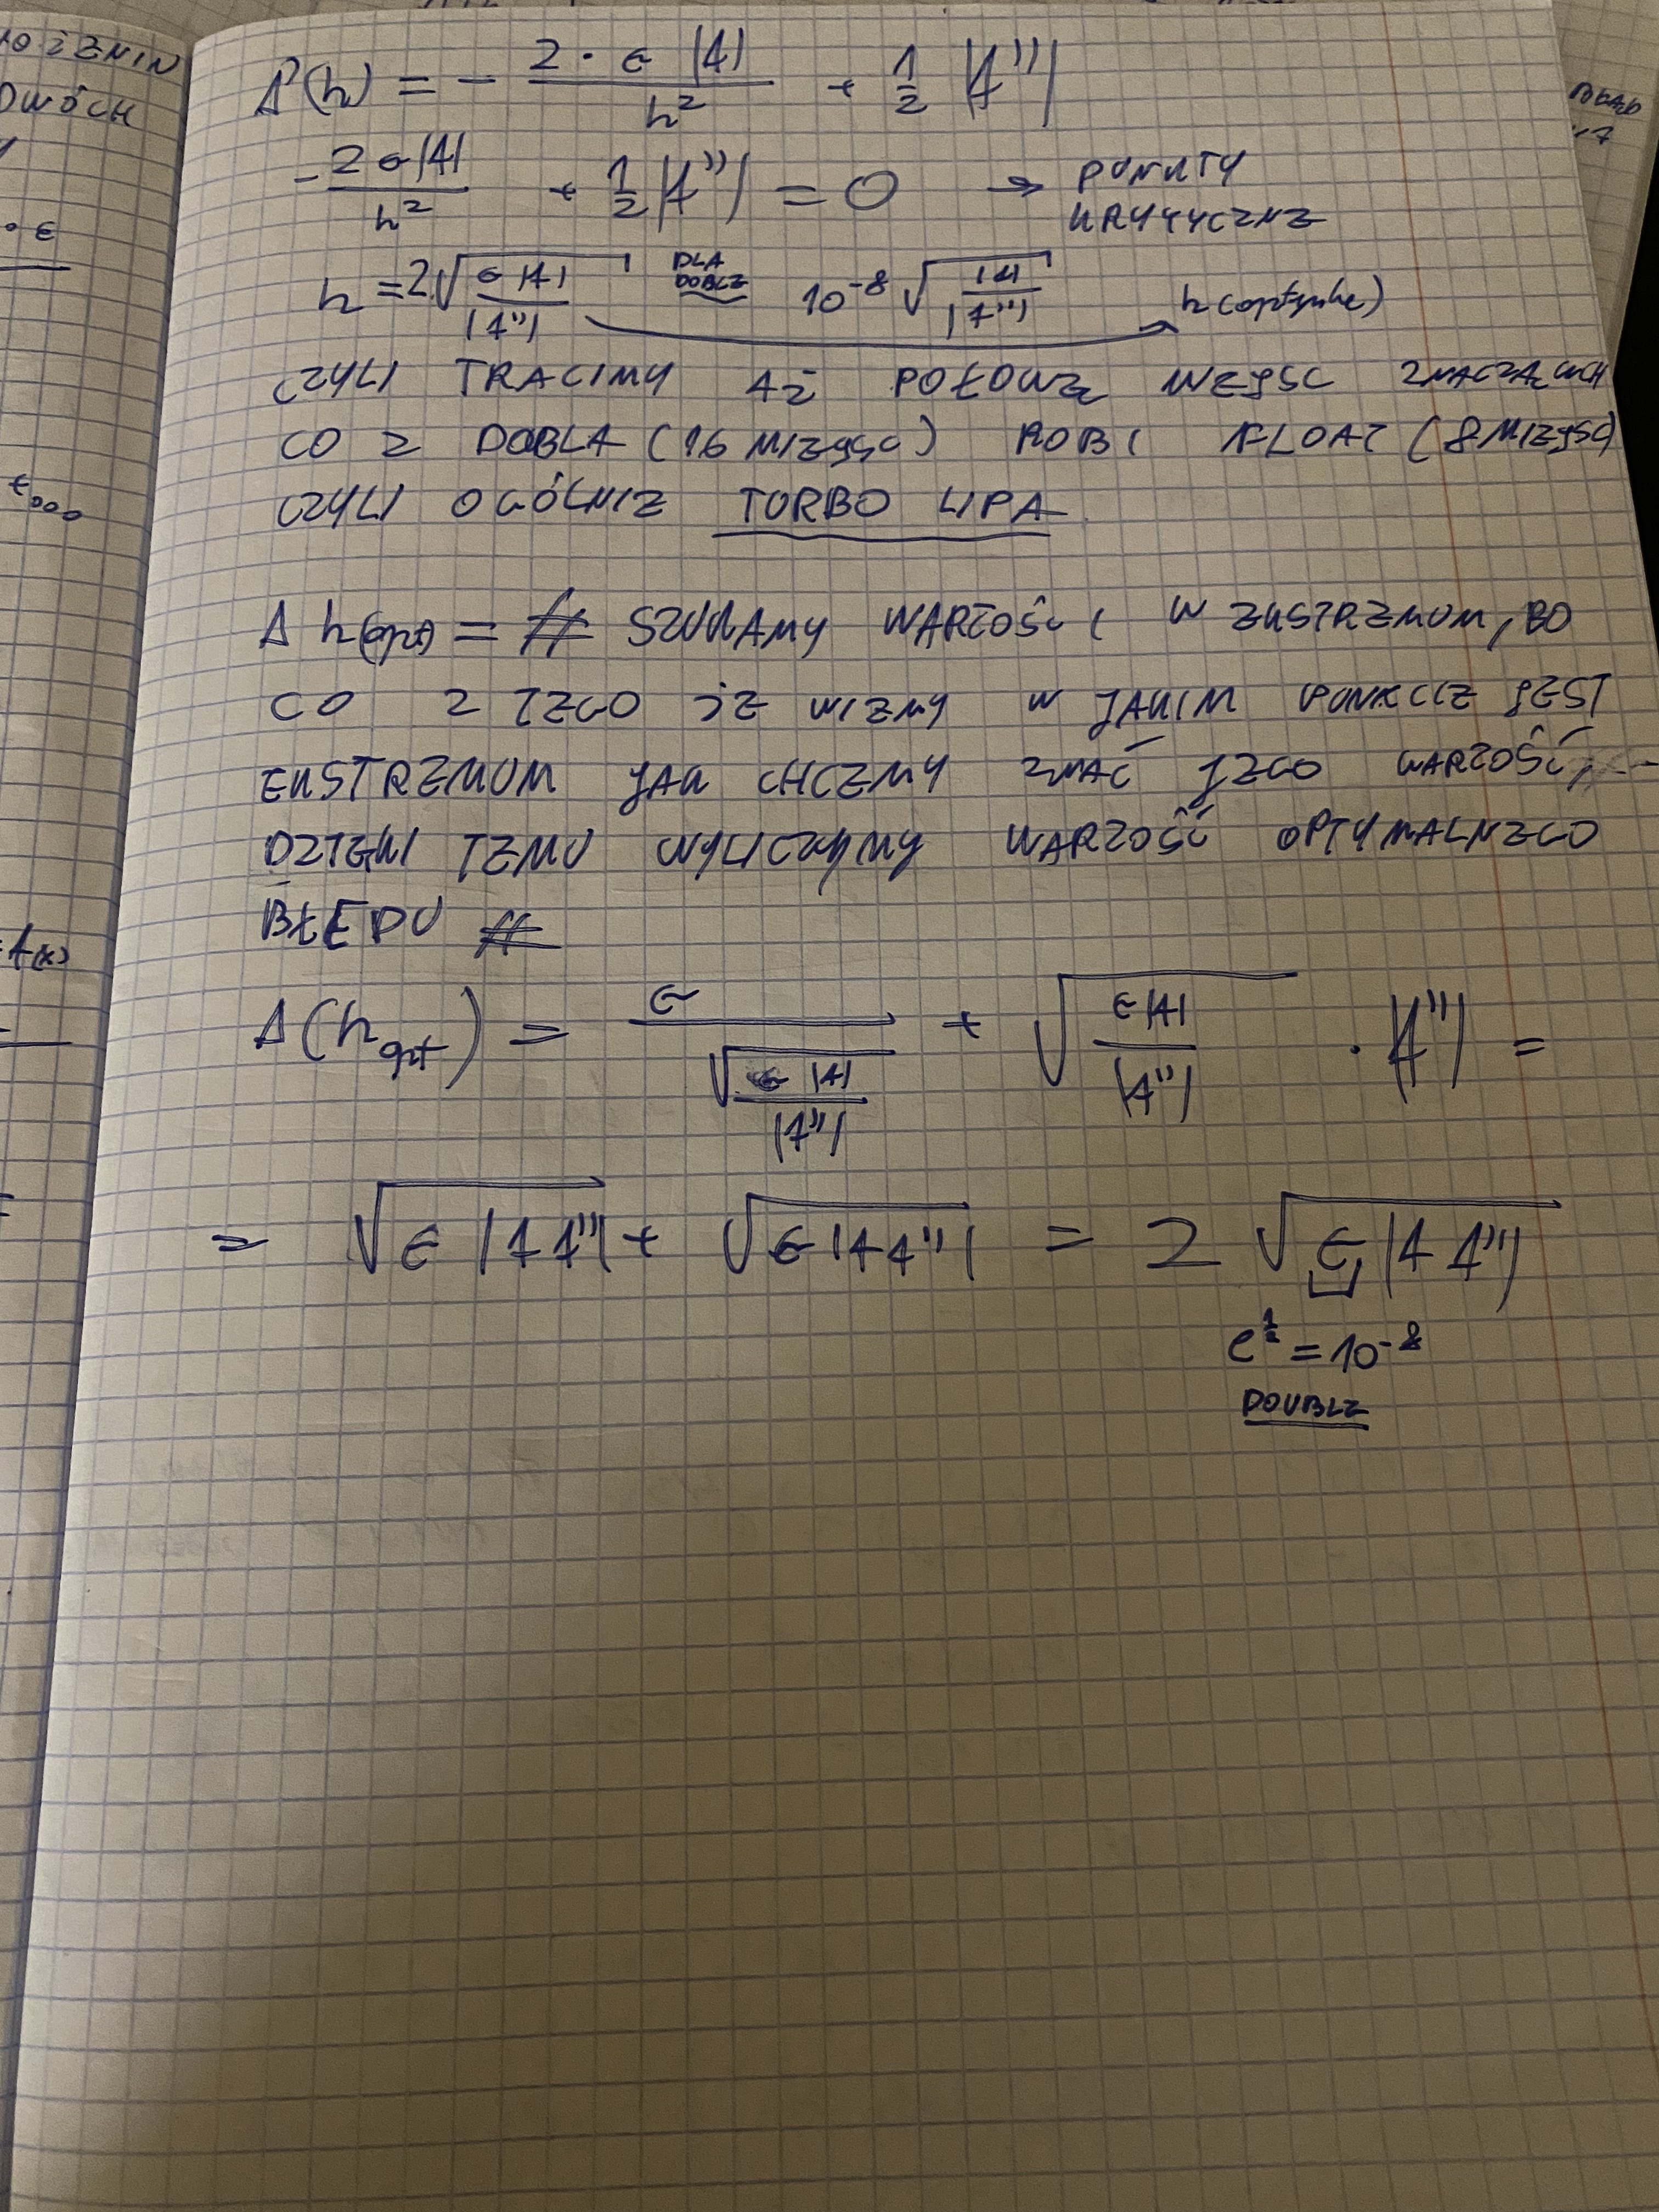
\includegraphics[width=10cm,height=10cm, keepaspectratio]{iloraz1}
\newline
\newline
\subsection{Analiza ilorazu B}
Dla drugiego wykresu(pierwszy rysnek iloraz B), nasz wykres spada do wartości minimalnej(h optymalne jest przyjmowane szybciej) szybciej niz wykres 1 oraz jego błąd optymalny jest mniejszy, bierze się to z tąd, że odejmujemy troche dalsze od siebie liczby bo $sin(x-h) - sin(x+h)$ to tak jakby odjac 1.98 do 2.02, jak widac moduł roznicy tych liczb jest większy niż liczb np 2.00 - 2.02, wiec błąd powinien nam zmaleć co stało się na wykresie drugim, ponieważ dodajemy troche większe od siebie liczby. Na polepszenie się wartości błedu wpływają również lekko większe liczby w mianowniku($2*h$). Ten błąd podobnie jak w przypadku pierwszym wynika z analizy szeregiem taylora, która załączam ponizej.
\newline
\newline
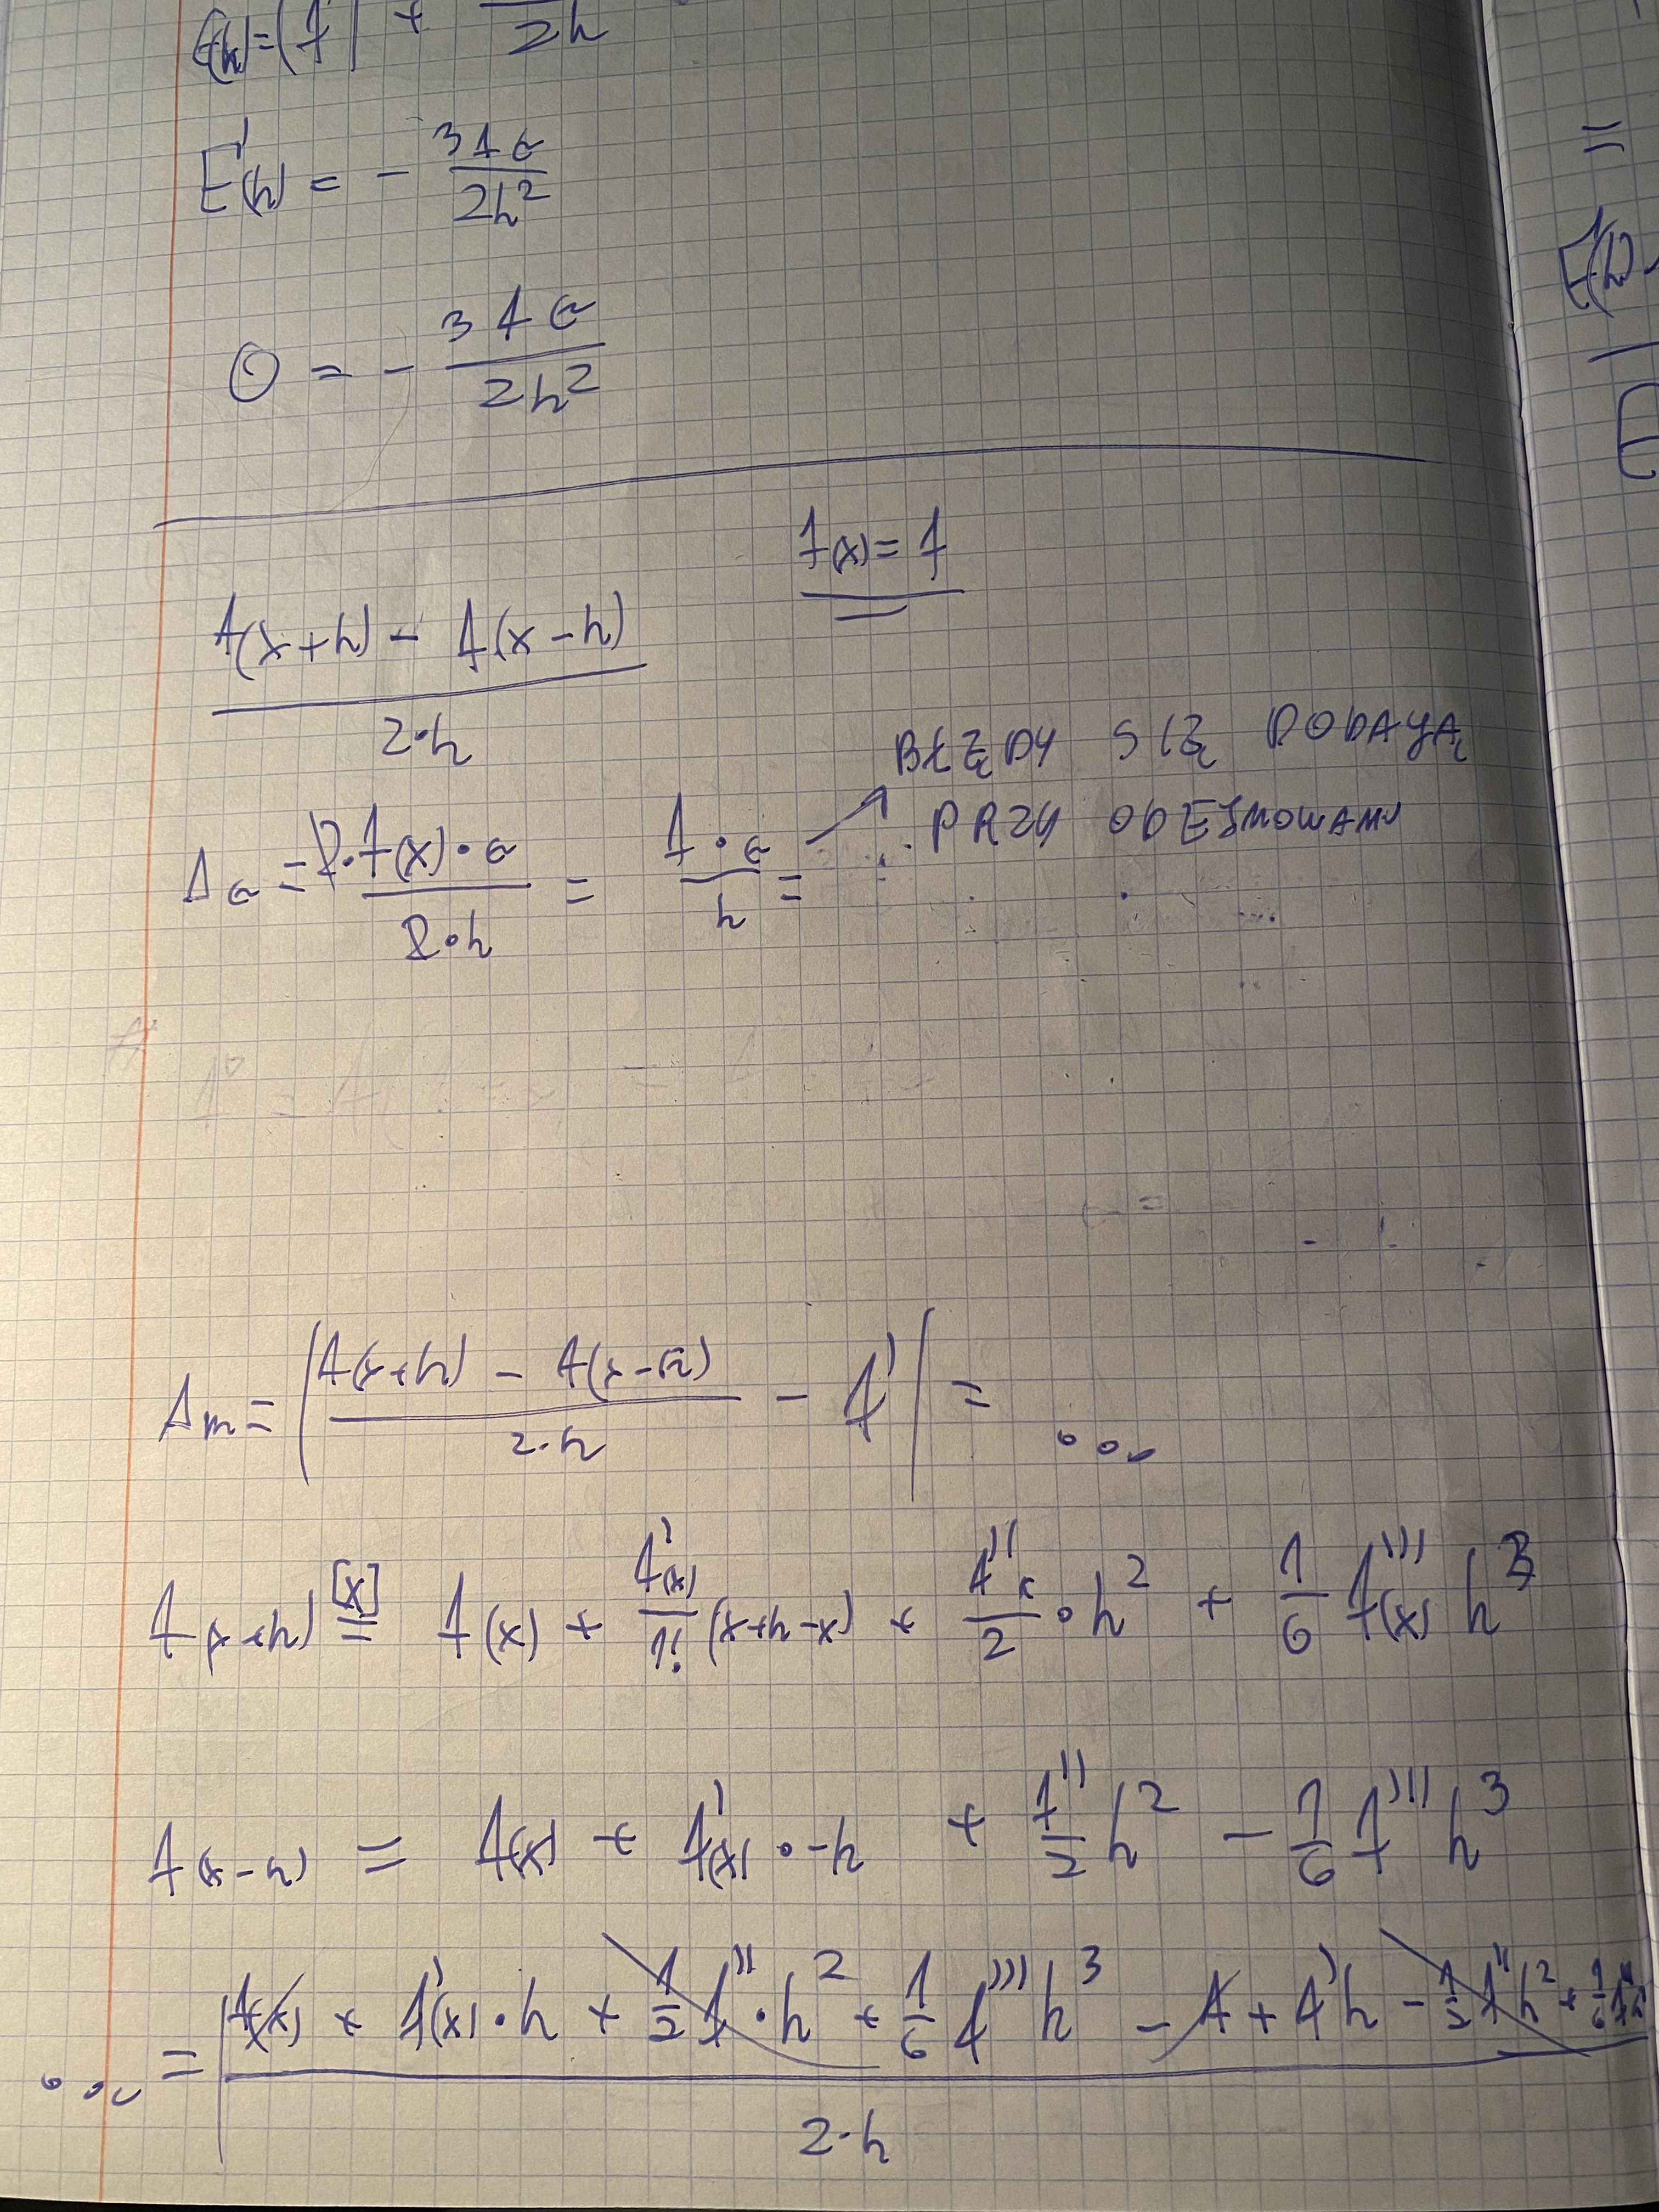
\includegraphics[width=10cm,height=10cm, keepaspectratio]{iloraz2_1.png}
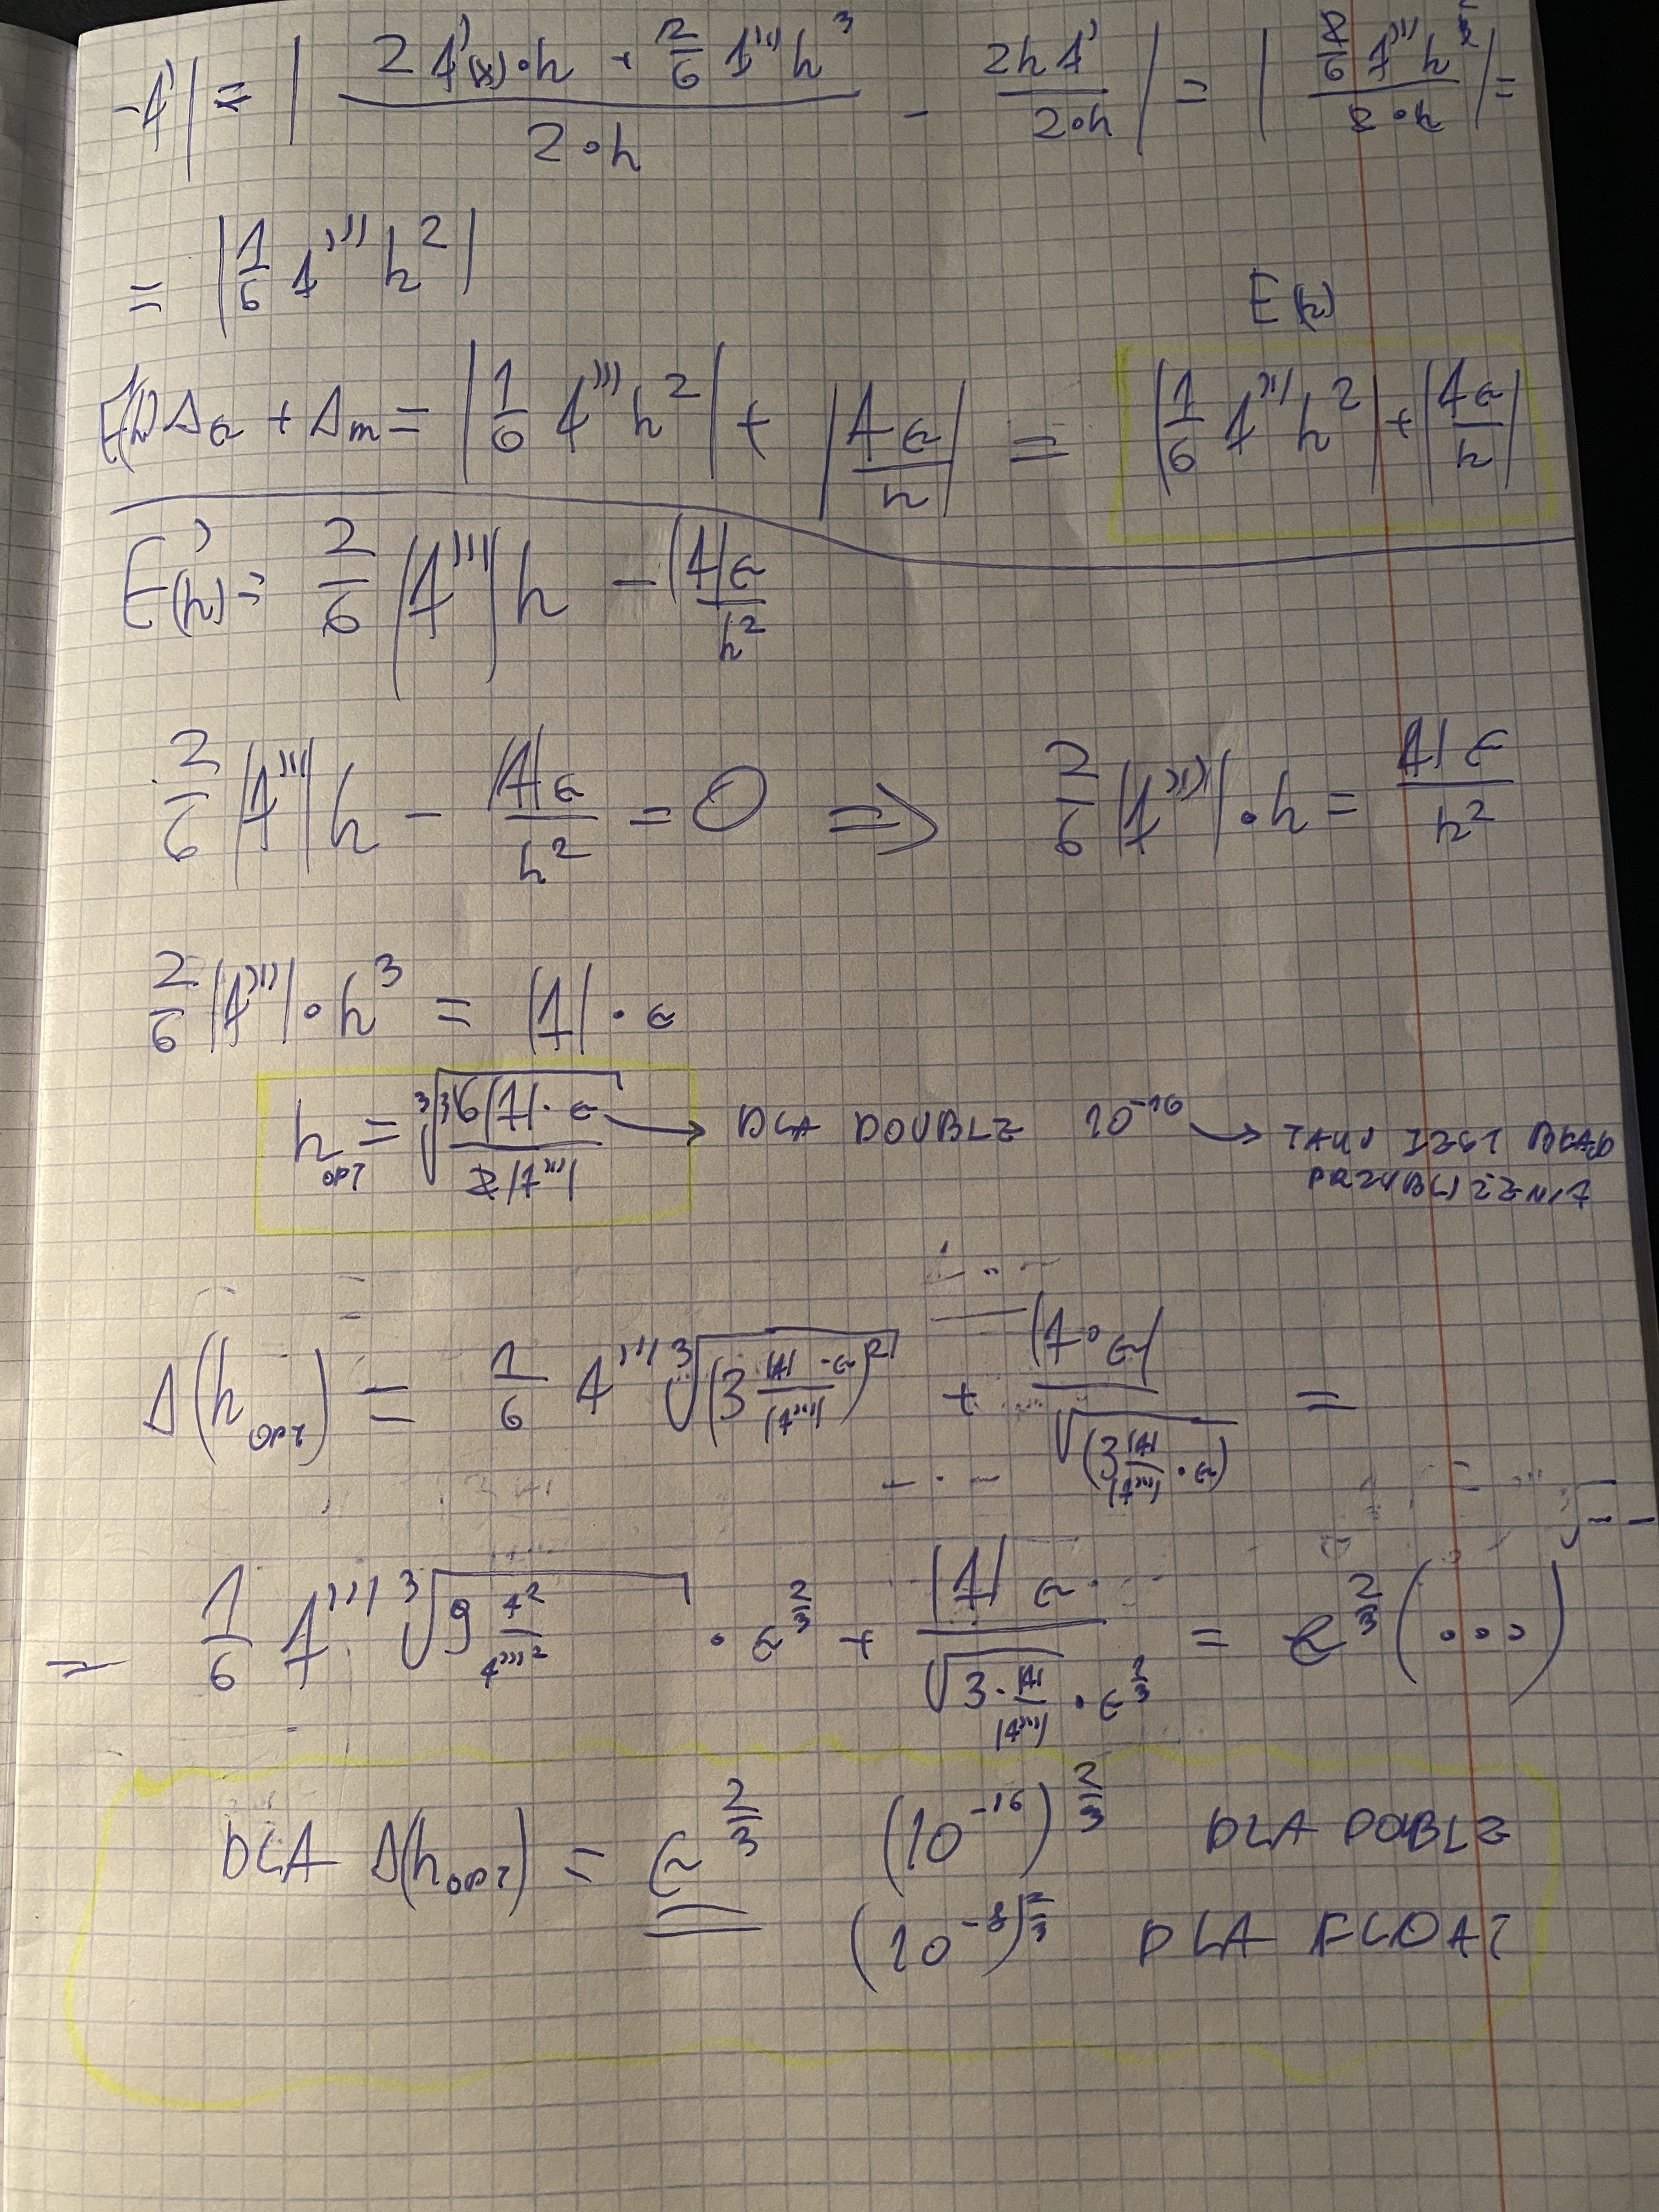
\includegraphics[width=10cm,height=10cm, keepaspectratio]{iloraz2_2.png}
\newline
\newline
\subsection{Analiza ilorazu C}
Teraz spójrzmy na wykres 3(pierwszy rysunek, iloraz C), który jest zdecydowanie najlepszy z nich wszystkich pod względem optymalnego błedu i szybkości zbiegania ku optymalnego h. Na trzecim przykładzie mamy już do czynienia z dośc dużym modułem różnicy liczb bo wyrażenie $-f(x + 2*h) + 8*f(x + h)$ bedzie dawało dużą różnice, to bardzo ładnie widać na wykresie tych funkcji, kiedy zaniebdamy sobie h, które zasadniczo przesuwa nam oba wykresy odrodinke w lewo jeśli h jest dodatnie lub w prawo kiedy h jest ujemne. Na wykresie można zauważyć(wykres ponizej), że nawet dla $x \approx 0$ bedziemy mieli odchylenie o wiele większe od wykresu funckji $8*sin(x)$ od $sin(x)$, ponieważ jest to pomnożone razy 8, jest to o wiele wiekszy odstep od liczb niż w przypadku ilorazu a i ilorazu b. Widzimy więc, że będziemy operować na liczbach względnie większych od poprzednich, co sprawia, że ten błąd będzie najmniejszy ze wszystkich. Na poprawę błędu wpływa również fakt, że dzielimy przez wiekszą liczbę bo $12*h$. .Również błąd wynika, z analizy szeregiem taylora. 
\newline
\newline
\includegraphics[width=15cm,height=15cm, keepaspectratio]{wykres_sin}
\newline
\newline
\subsection{Analiza dla float}
Teraz jeszcze wspomne dlaczego wykresy(rysunek drugi i wszystkie na nim wykresy) troche roznia sie w zaleznosci od precyzji jaką przyjmiemy; uogolniajac, to rowniez wynika z analizy taylorowskiej, bo podstawiwszy np nasze epsilon rowne $10^{-8}$ dla float dostaniemy dla pierwszego ilorazu epsilon rowne $10^{-4}$ to sie pokrywa mniej więcej z otrzymanym minimum wykresu. Tłumaczac co sie dzieje dla bardzo malych h, to tak naprawde tracimy w pewnym momencie dostepna nam precyzje i wykraczamy poza jej zakres przez co dzielimy przez 0 co sprawia ze z wykresem dzieją się dziwne rzeczy, ale jeśli sobie przyblizymy to zobaczymy ze wykres zachowuje sie tak samo jak dla double przez pewien przedzial h(h jest zazwyczaj z przedziału precyzji, czyli wykres bedzie zachowywał się normalnie od $h \in [10^{-8} , ...]$ - dla float i dla double $h \in [10^{-16} , ...]$).
\newline
\newline
\section{Próba analizy, co dzieje się z punktem x = $\frac{\pi}{2}$}
\subsection*{Float}
\includegraphics[width=15cm,height=15cm, keepaspectratio]{wykres_float_pi}
\subsection*{Double}
\includegraphics[width=15cm,height=15cm, keepaspectratio]{wykres_double_pi}
Teraz rozwazmy dlaczego nasze wykresy wygladaja tak dziwnie dla punktu $\frac{\pi}{2}$. 
Po pierwsze jak wiemy $cos(\frac{\pi}{2}) \approx 0$, wiec bedziemy odejmowac podczas liczenia bledu obliczania limesa, naszą wartość z ilorazu i 0. Teraz mozemy podstawic odpowiednio $\frac{\pi}{2}$ do naszej funkcji błędu i dostajemy, ze:
\newline
\newline
\begin{center}
    $\frac{sin(\frac{\pi}{2} + h) - sin(\frac{\pi}{2})}{2*h}$
    \newline
    \newline
\end{center}
bedziemy mieli ze $sin(\frac{\pi}{2} + h) \approx 1$ oraz $sin(\frac{\pi}{2}) \approx 1$ oraz $cos(\frac{\pi}{2}) \approx 0$ (przez blad numeryczny przyblizenia pi, nie dostaniemy dokladnej wartosci rownej 0), daje nam to specyficzne rownanie, z ktorego mozemy wywnioskowac, ze dla odpowiednio maly h, blad ten bedzie praktycznie rowny zero. Wiec mozna powiedziec, ze zaniedbamy sobie nasz blad maszynowy wynikający z liczenia limesa. Ale zostal nam jeszcze blad zapisu, który juz sie nie zniesie, on zostanie i bedzie wynosil $\approx \frac{\epsilon*sin(\frac{\pi}{2})}{h}$, tak naprawde blad ten dla odpowiednio malego h to poprostu bedzie $\epsilon$, wiec z tad ta stala praktycznie kreska na dole w okolicach prezycji double i float, ale taki skok przy odpowiednio duzym h, wynika z tego, ze tak jak poprzednio, oddalamy sie od naszej granicy w zerze i nasz wykres zaczyna rosnąć.
\section{Wartości $h_{opt}$ dla odpowiednich ilorazów:}
\subsection*{Zaczne od punktu $x = \frac{\pi}{2}$ (wartość błedu optymalnego będe oznaczać poprzez $E(h_{opt})$):}
Dla precyzji float oraz ilorazu A, B, C dostaniemy odpowiednio precyzje float czyli $E(x) \approx 10^{-8}$
\newline
\newline
Dla precyzji double oraz ilorazu A, B, C dostaniemy odpowiednio precyzje double czyli $E(x) \approx 10^{-16}$
\newline
\newline
\subsection*{Teraz przejdzmy do punktu x = 1:}
Dla precyzji double mamy odpowiednio:
\begin{itemize}
    \item Iloraz A: $h_{opt} \approx 1.4 * 10^{-8}$ oraz $E(h_{opt}) \approx 10^{-9}$
    \item Iloraz B: $h_{opt} \approx 6 * 10^{-6}$ oraz $E(h_{opt}) \approx 10^{-12}$
    \item Iloraz C: $h_{opt} \approx  10^{-3}$ oraz $E(h_{opt}) \approx 10^{-14}$
\end{itemize}
Dla precyzji float mamy odpowiednio:
\begin{itemize}
    \item Iloraz A: $h_{opt} \approx 1.7 * 10^{-4}$ oraz $E(h_{opt}) \approx 10^{-4}$
    \item Iloraz B: $h_{opt} \approx 4 * 10^{-3}$ oraz $E(h_{opt}) \approx 10^{-7}$
    \item Iloraz C: $h_{opt} \approx 5^{-2}$ oraz $E(h_{opt}) \approx 6*10^{-8}$
\end{itemize}









\end{document}